% !TeX root=../main.tex

\chapter{نتایج}
\label{ch:results}

\section{مقدمه}
این فصل نتایج تجربی حاصل از ۱۶۰ اجرای ریزتنظیم مستقل (بخش~\ref{sec:ablation}) به‌علاوهٔ ارزیابی خط پایهٔ مدل پیش‌آموزش‌دیده را گزارش می‌کند. ترتیب ارائه به این صورت است: ابتدا اثر شرط آزمایشی و وزن
$\lambda$ (بخش~\ref{sec:res-condition})، پس‌ازآن اثر انتخاب لایهٔ هدف (بخش~\ref{sec:res-layer})، هزینهٔ این بهبود از نظر سرگشتگی زبانی و اعتبار خودرمزگذار (بخش~\ref{sec:res-dynamics})، و سرانجام معرفی یک پیکربندی توصیه‌شده بر مبنای مصالحهٔ میان این دو (بخش~\ref{sec:res-best}).

% \section{خط پایه}
% \label{sec:res-baseline}
% پیش از هرگونه ریزتنظیم، مدل پیش‌آموزش‌دیده روی شکاف آزمون
% \lr{PAWS}
% در تمام لایه‌ها ارزیابی شد. شکل~\ref{fig:baseline} این خط پایه را نشان می‌دهد.

% \begin{figure}[htb]
% \centering
% 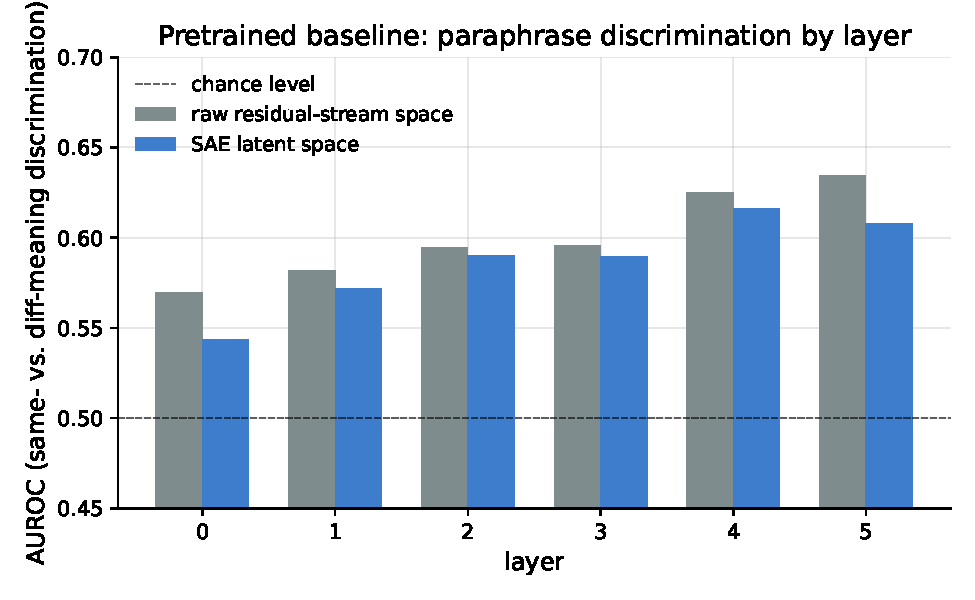
\includegraphics[width=0.8\textwidth]{baseline_auroc_by_layer}
% \caption{\lr{AUROC} خط پایه (مدل پیش‌آموزش‌دیده، بدون ریزتنظیم) در فضای خام و فضای \lr{SAE}، به ازای هر یک از لایه‌های مدل.}
% \label{fig:baseline}
% \end{figure}

% دو مشاهده در این نمودار قابل‌توجه است. نخست،
% \lr{AUROC}
% در هر دو فضا، در تمام لایه‌ها، بالاتر از سطح حدس تصادفی
% (۵٫۰)
% اما فاصلهٔ چندانی از آن ندارد؛ به بیان دیگر، حتی بدون هیچ ریزتنظیمی، مدل تا حدی جفت‌های هم‌معنی و ناهم‌معنی
% \lr{PAWS}
% را از هم متمایز می‌کند، اما این تمایز به‌هیچ‌وجه قوی نیست. دوم، و مهم‌تر برای این پژوهش:
% $\Delta_{\mathrm{AUROC}} = \mathrm{AUROC}_{\mathrm{SAE}} - \mathrm{AUROC}_{\mathrm{raw}}$
% در تمام لایه‌ها منفی است. این یافته، فرض اولیهٔ ساده‌انگارانه‌ای را که می‌شد پیش‌آموزش داشت--اینکه فضای
% \lr{SAE}
% به‌طور ذاتی و بدون هیچ مداخله‌ای، تفکیک‌کنندهٔ بهتری از معنا باشد--رد می‌کند: در مدل خام و پیش‌آموزش‌دیده، عبوردادن فعال‌سازی‌ها از خودرمزگذار، نه‌تنها کمکی به تفکیک هم‌معنی/ناهم‌معنی نمی‌کند، بلکه اندکی هم آن را بدتر می‌کند؛ احتمالاً چون خطای بازسازی خود خودرمزگذار (که هیچ‌گاه صفر نیست) بخشی از سیگنال ظریف لازم برای این تفکیک را از بین می‌برد. این مشاهده، پرسش اصلی این پایان‌نامه را برجسته‌تر می‌کند: آیا می‌توان با ریزتنظیم هدفمند، این رابطه را معکوس کرد؟

\section{اثر شرط آزمایشی و وزن ناوردایی}
\label{sec:res-condition}
برای هر یک از ۱۶۰ اجرا، بهبود
\lr{AUROC}
در فضای
\lr{SAE}
نسبت به خط پایه، در همان لایه(ها)یی که هدف تابع هزینهٔ ناوردایی بوده‌اند، محاسبه شد. جدول~\ref{tab:cond-summary} میانگین این بهبود را--با میانگین‌گیری روی تمام ده حالت انتخاب لایه و (برای شرایط دارای
$\lambda$) روی هر پنج مقدار آن--برای هر شرط خلاصه می‌کند.

\begin{table}[htb]
\centering
\caption{میانگین و بازهٔ بهبود \lr{AUROC} نسبت به خط پایه، در لایه(های) هدف، به تفکیک شرط آزمایشی.}
\label{tab:cond-summary}
\begin{tabular}{lrrr}
\toprule
شرط & میانگین بهبود & کمینه & بیشینه \\
\midrule
\lr{C1} (کنترل، بدون ناوردایی) & $-0.0014$ & $-0.0067$ & $+0.0012$ \\
\lr{C2} (ناوردایی، فضای خام) & $-0.0008$ & $-0.0204$ & $+0.0253$ \\
\lr{C3} (ناوردایی، فضای \lr{SAE}) & $+0.0129$ & $-0.0347$ & $+0.0694$ \\
\lr{C4} (فضای \lr{SAE} + حمایت) & $+0.0150$ & $-0.0336$ & $+0.0678$ \\
\bottomrule
\end{tabular}
\end{table}

سه یافتهٔ این جدول، ستون فقرات اصلی نتایج این پایان‌نامه‌اند. نخست،
\lr{C1}--شرط کنترلی که هیچ سیگنالی از
\lr{PAWS}
دریافت نمی‌کند--میانگین بهبودی تقریباً صفر (و اندکی منفی) دارد؛ این تأیید می‌کند که صرف ریزتنظیم‌کردن مدل روی
\lr{WikiText}، به‌خودی‌خود، جداسازی هم‌معنی/ناهم‌معنی را بهبود نمی‌بخشد. دوم،
\lr{C2}--اعمال همان تابع هزینهٔ ناوردایی، اما در فضای خام--نیز به‌طور میانگین تفاوت معناداری با خط پایه ندارد، هرچند واریانس آن به‌مراتب بیشتر از
\lr{C1}
است: اعمال این هدف مستقیماً در فضای خام گاهی کمی کمک می‌کند و گاهی کمی ضرر می‌رساند، بدون الگویی قابل‌اتکا. سوم، و مهم‌ترین یافته: تنها با انتقال همین تابع هزینه به فضای
\lr{SAE}
(شرایط
\lr{C3}
و
\lr{C4}) میانگین بهبود به‌طور قابل‌توجهی مثبت می‌شود، و بیشینهٔ بهبود در بهترین پیکربندی‌ها به نزدیک
۰۷٫۰
می‌رسد. این تباین سه‌گانه--کنترل خنثی، فضای خام بی‌اثر، فضای
\lr{SAE}
مؤثر--شاهد تجربی اصلی این پایان‌نامه به نفع فرضیهٔ محوری آن است: خودرمزگذار پراکنده، فضای مؤثرتری برای شکل‌دادن این نوع بازنمایی فراهم می‌کند. جزء حمایتی تکمیلی
\lr{C4}
نسبت به
\lr{C3}
اندکی بهتر عمل می‌کند، هرچند این تفاوت در مقایسه با شکاف اصلی میان فضای خام و فضای
\lr{SAE}، کوچک است. \emph{مقادیر بیشینهٔ جدول بالا--که همگی در وزن $\lambda$ بزرگ به دست می‌آیند--را باید با احتیاط خواند: همان‌طور که در بخش~\ref{sec:res-dynamics} نشان داده می‌شود، این مقادیر با هزینه‌ای در پایداری آموزش همراه‌اند که در همین جدول دیده نمی‌شود.}

شکل~\ref{fig:gain-vs-lambda} همین دادگان را به‌تفکیک وزن $\lambda$ نشان می‌دهد.

\begin{figure}[htb]
\centering
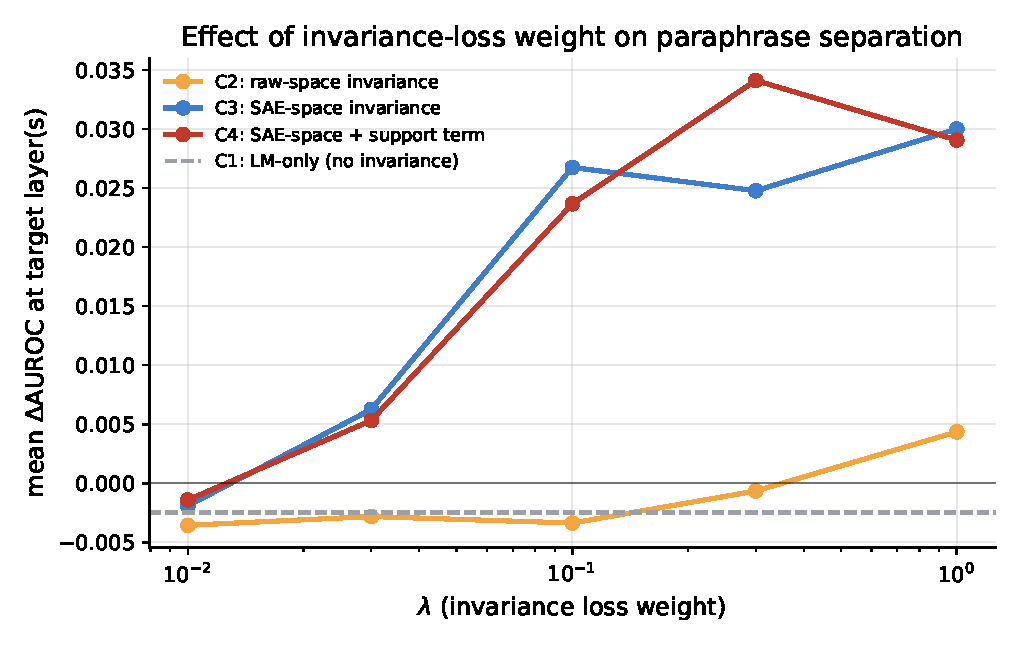
\includegraphics[width=0.85\textwidth]{gain_vs_lambda}
\caption{میانگین بهبود \lr{AUROC} در لایه(های) هدف، بر حسب وزن تابع هزینهٔ ناوردایی $\lambda$ (میانگین روی هر ده حالت انتخاب لایه). خط افقی، سطح شرط \lr{C1} (فاقد $\lambda$) را نشان می‌دهد.}
\label{fig:gain-vs-lambda}
\end{figure}

الگوی این نمودار برای
\lr{C3}
و
\lr{C4}
تقریباً یکسان است: در $\lambda = 0.01$، بهبود عملاً صفر یا منفی است--یعنی سیگنال ناوردایی در برابر هزینهٔ زبان‌مدل‌سازی چنان ضعیف است که عملاً بی‌اثر می‌ماند. با رسیدن $\lambda$ به $0.1$، جهش محسوسی در بهبود رخ می‌دهد، و از آن پس، افزایش بیشتر $\lambda$ تا $1.0$ سود نسبتاً کمی به همراه دارد. در مقابل، برای
\lr{C2} (فضای خام)، حتی در $\lambda = 1.0$ بهبود میانگین ناچیز باقی می‌ماند. جدول کامل این ارقام، به تفکیک هر مقدار $\lambda$، در پیوست «ب» آمده است؛ همان‌طور که در بخش~\ref{sec:res-dynamics} نشان داده خواهد شد، رفتن به سمت  $\lambda$ بزرگ برای کسب همین سود نهایی، هزینه‌ای در پایداری آموزش دارد که ارزش آن را باید در کنار اندازهٔ بهبود سنجید.

\section{اثر انتخاب لایهٔ هدف و نمایهٔ کامل عمق}
\label{sec:res-layer}
محور دوم آزمایش‌های شبکه‌ای، انتخاب لایه(های) هدف بود. شکل~\ref{fig:gain-layers} دو جنبهٔ این محور را نشان می‌دهد: تأثیر \emph{تعداد} لایه‌های هم‌زمان و تأثیر اینکه \emph{کدام} لایهٔ منفرد انتخاب شده، هر دو با میانگین‌گیری روی شرایط
\lr{C3}
و
\lr{C4}
و تمام مقادیر $\lambda$.

\begin{figure}[htb]
\centering
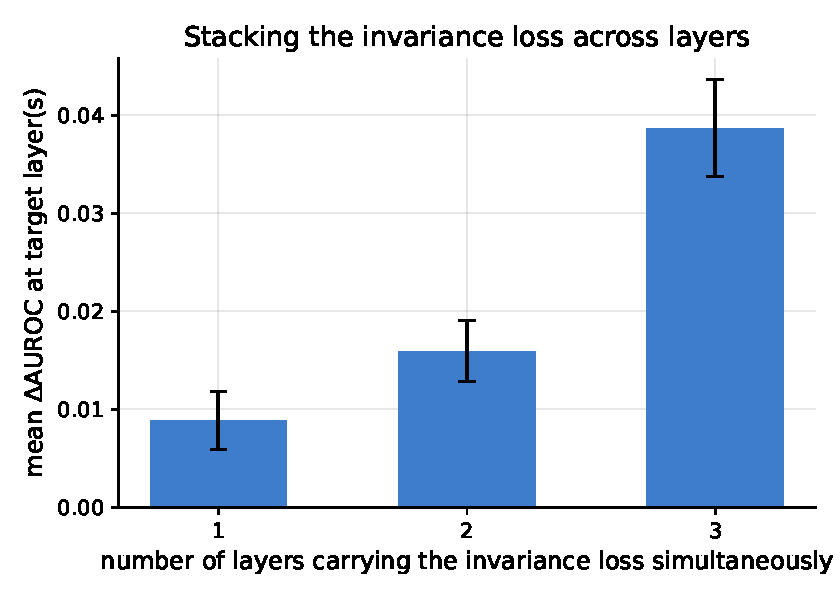
\includegraphics[width=0.48\textwidth]{gain_by_n_layers}
\hfill
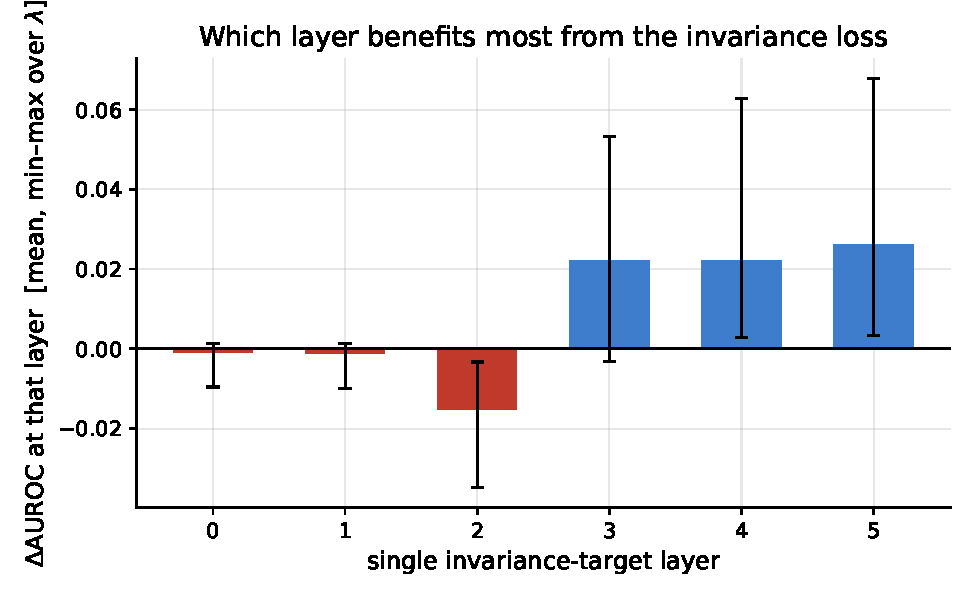
\includegraphics[width=0.48\textwidth]{gain_by_target_layer}
\caption{چپ: میانگین بهبود \lr{AUROC} بر حسب اینکه کدام لایهٔ \emph{منفرد} هدف تابع هزینهٔ ناوردایی بوده (میله‌های خطا، بازهٔ کمینه تا بیشینه روی $\lambda$ها را نشان می‌دهند). راست: میانگین بهبود بر حسب \emph{تعداد} لایه‌هایی که هم‌زمان تحت تابع هزینهٔ ناوردایی قرار گرفته‌اند. هر دو نمودار، میانگین شرایط \lr{C3} و \lr{C4} است.}
\label{fig:gain-layers}
\end{figure}

نمودار سمت چپ الگویی غیریکنواخت اما معنادار را آشکار می‌کند: لایه‌های نزدیک به ورودی تقریباً بی‌اثرند؛ لایهٔ دوم (از شش لایهٔ مدل) به‌طور سیستماتیک \emph{زیان‌آور} است (بدترین مورد منفرد کل این پایان‌نامه، دقیقاً در همین لایه رخ داده است)؛ و از حدود نیمهٔ عمق مدل به بعد، بهبود به‌طور پیوسته مثبت و رو به افزایش است. به‌عبارت دیگر، اعمال هدف ناوردایی روی لایه‌های ابتدایی این مدل کوچک، در بهترین حالت بی‌فایده و در بدترین حالت مخرب است؛ درحالی‌که همین هدف، وقتی روی نیمهٔ دوم عمق مدل اعمال شود، به‌طور پایدار سودمند است. این الگو با این تعبیر رایج در ادبیات تفسیرپذیری سازگار است که لایه‌های ابتدایی یک مدل زبانی عمدتاً بازنمایی سطحی و واژگانی می‌سازند، درحالی‌که بازنمایی معنایی و ترکیبی--که برای تشخیص تفاوت ظریف میان جفت‌جمله‌های
\lr{PAWS}
لازم است--در لایه‌های عمیق‌تر شکل می‌گیرد.

نمودار سمت راست نشان می‌دهد که اثر اعمال هم‌زمان تابع هزینه روی چند لایه، نه‌تنها جمع‌شونده بلکه فراجمع‌شونده\LTRfootnote{Super-additive}
است: میانگین بهبود برای سه لایهٔ هم‌زمان، به‌وضوح بیش از سه برابر میانگین بهبود یک لایهٔ منفرد است. تعبیر محتمل این است که چون جریان باقیمانده در معماری ترنسفورمر جمعی\LTRfootnote{Additive}
است، اعمال هم‌زمان هدف روی چند لایهٔ متوالی، مسیرهای بیشتری برای شکل‌دادن دوبارهٔ محاسبات درونی مدل در جهت هدف موردنظر در اختیار بهینه‌سازی می‌گذارد.

شکل~\ref{fig:profile} نمایهٔ کامل عمق پیکربندی با شرط
\lr{C3}
با هدف‌گیری هم‌زمان لایه‌های $\{3,4,5\}$ و $\lambda=1.0$ را در برابر خط پایه نشان می‌دهد.

\begin{figure}[htb]
\centering
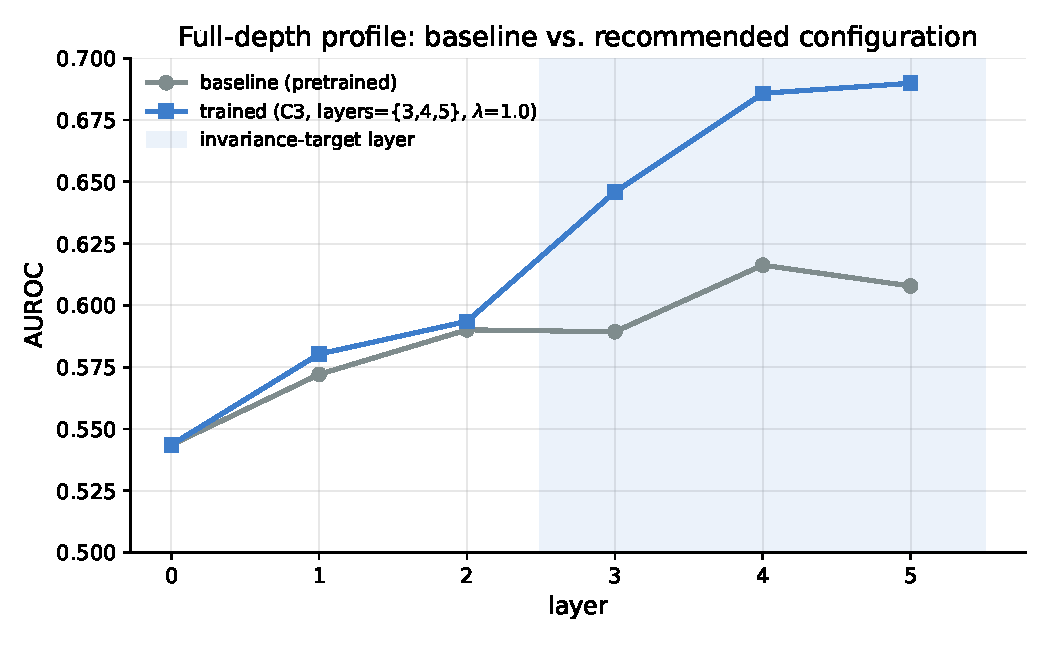
\includegraphics[width=0.85\textwidth]{profile_best_vs_baseline}
\caption{نمایهٔ کامل \lr{AUROC} در تمام شش لایه، برای خط پایه در برابر بهترین پیکربندی (\lr{C3}، لایه‌های هدف $\{3,4,5\}$، $\lambda=1.0$). ناحیهٔ سایه‌خورده، لایه‌های هدف را نشان می‌دهد.}
\label{fig:profile}
\end{figure}

نکتهٔ مهم این نمایه، رفتار آن در لایه‌های \emph{غیرهدف} (۰ تا ۲) است: بهبود در این لایه‌ها عملاً ناچیز اما مثبت است ($+0.00$ در لایهٔ ۰ تا $+0.008$ در لایهٔ ۱)، نه منفی. به‌عبارت دیگر، فشاردادن بازنمایی لایه‌های عمیق در جهت جداسازی بهتر هم‌معنی/ناهم‌معنی، به‌بهای تخریب بازنمایی لایه‌های کم‌عمق‌تر تمام نشده است؛ این تعمیم‌ناپذیری خوش‌خیم (نه مثبت و نه منفی محسوس) نشان می‌دهد اثر آموزش، تا حد زیادی موضعی و محدود به همان لایه‌هایی است که مستقیماً هدف قرار گرفته‌اند.

الگوی مشابهی، با جزئیات بیشتر، در بهترین پیکربندی \emph{تک‌لایه} (لایهٔ ۵، شرط
\lr{C4}، $\lambda=0.3$، با بهبود $+0.068$ در همان لایه) دیده می‌شود: بهبود در لایه‌های ۰ تا ۳ عملاً صفر است (کمتر از $0.001$ در قدرمطلق)، اما در لایهٔ ۴--که مستقیماً هدف قرار نگرفته، ولی بلافاصله \emph{پیش از} لایهٔ هدف قرار دارد--بهبود قابل‌توجه $+0.043$ ثبت شده است. این «نشت» بهبود به‌سمت عقب، با معماری جریان باقیماندهٔ ترنسفورمر سازگار است: فعال‌سازی لایهٔ ۵، تابعی مستقیم از فعال‌سازی لایهٔ ۴ است، و بنابراین، هر تغییری که وزن‌های لورا برای دورکردن بازنمایی لایهٔ ۵ اعمال می‌کنند، الزاماً بازنمایی لایهٔ ۴ (که ورودی لایهٔ ۵ را می‌سازد) را نیز تحت‌تأثیر قرار می‌دهد. این یافته پیشنهاد می‌کند که تعمیم اثر این روش، بیشتر «رو به عقب» (به لایه‌های نزدیک‌تر به ورودی که خروجی‌شان مستقیماً وارد لایهٔ هدف می‌شود) رخ می‌دهد تا «رو به جلو».

\section{هزینهٔ پایداری: سرگشتگی و اعتبار خودرمزگذار}
\label{sec:res-dynamics}
نتایج دو بخش پیشین، عمداً تنها بهبود نهایی
\lr{AUROC}
را گزارش کردند. اما این بهبود، رایگان به دست نیامده است. این بخش دو سنجهٔ سلامت جانبی--سرگشتگی زبانی و اعتبار بازسازی خودرمزگذار--را در سرتاسر شبکهٔ آزمایشی بررسی می‌کند.

\subsection{سرگشتگی زبان‌مدل‌سازی}
جدول~\ref{tab:ppl} میانگین سرگشتگی اعتبارسنجی
\lr{WikiText}
را در گام پایانی آموزش، به‌تفکیک شرط و $\lambda$، نشان می‌دهد.

\begin{table}[htb]
\centering
\caption{میانگین سرگشتگی \lr{WikiText} در گام پایانی آموزش، به تفکیک شرط و $\lambda$. برای مقایسه، شرط \lr{C1} (بدون هیچ هدف ناوردایی) به سرگشتگی $59.1$ می‌رسد.}
\label{tab:ppl}
\begin{tabular}{lccc}
\toprule
$\lambda$ & \lr{C2} (خام) & \lr{C3} (\lr{SAE}) & \lr{C4} (\lr{SAE}+حمایت) \\
\midrule
$0.01$ & $59.0$ & $59.2$ & $59.1$ \\
$0.03$ & $59.1$ & $59.1$ & $59.4$ \\
$0.10$ & $59.1$ & $60.2$ & $59.9$ \\
$0.30$ & $59.5$ & $65.9$ & $64.4$ \\
$1.00$ & $67.5$ & $89.0$ & $84.4$ \\
\bottomrule
\end{tabular}
\end{table}

الگوی این جدول واضح است: تا
$\lambda=0.1$، سرگشتگی در تمام شرایط عملاً دست‌نخورده می‌ماند (در محدودهٔ
\lr{59}
تا
\lr{60}، تقریباً برابر با شرط کنترلی). از
$\lambda=0.3$
به بعد، شرایط
\lr{C3}
و
\lr{C4}--یعنی دقیقاً همان شرایطی که در فضای
\lr{SAE}
عمل می‌کنند--شروع به افزایش محسوس سرگشتگی می‌کنند، و در
$\lambda=1.0$، این افزایش به بیش از یک‌ونیم برابر (برای
\lr{C4}) تا نزدیک به سه برابر (برای
\lr{C3}) مقدار کنترلی می‌رسد. شرط
\lr{C2} (فضای خام) در برابر این اثر تا حد زیادی مصون است و تنها در
$\lambda=1.0$
افزایش ملایمی نشان می‌دهد. این عدم‌تقارن میان
\lr{C2}
و
\lr{C3}/\lr{C4}
با فرمول تابع هزینهٔ بخش~\ref{sec:loss} سازگار است: در شرایط
\lr{C3}
و
\lr{C4}، همان لایه‌ای که هدف تابع هزینهٔ ناوردایی است، همزمان ورودی خودرمزگذار نیز هست، و کشیده‌شدن این لایه در جهت جداسازی هم‌معنی/ناهم‌معنی، با حفظ سلامت عمومی زبانی--که به‌طور جداگانه و با وزن ثابت در تابع هزینه حضور دارد--به رقابت می‌افتد.

برای دیدن این مصالحه در سطح کل شبکهٔ آزمایشی--نه فقط میانگین‌های جدول بالا--شکل~\ref{fig:tradeoff} بهبود
\lr{AUROC}
هر یک از ۱۶۰ اجرا را در برابر سرگشتگی نهایی همان اجرا رسم می‌کند.

\begin{figure}[htb]
\centering
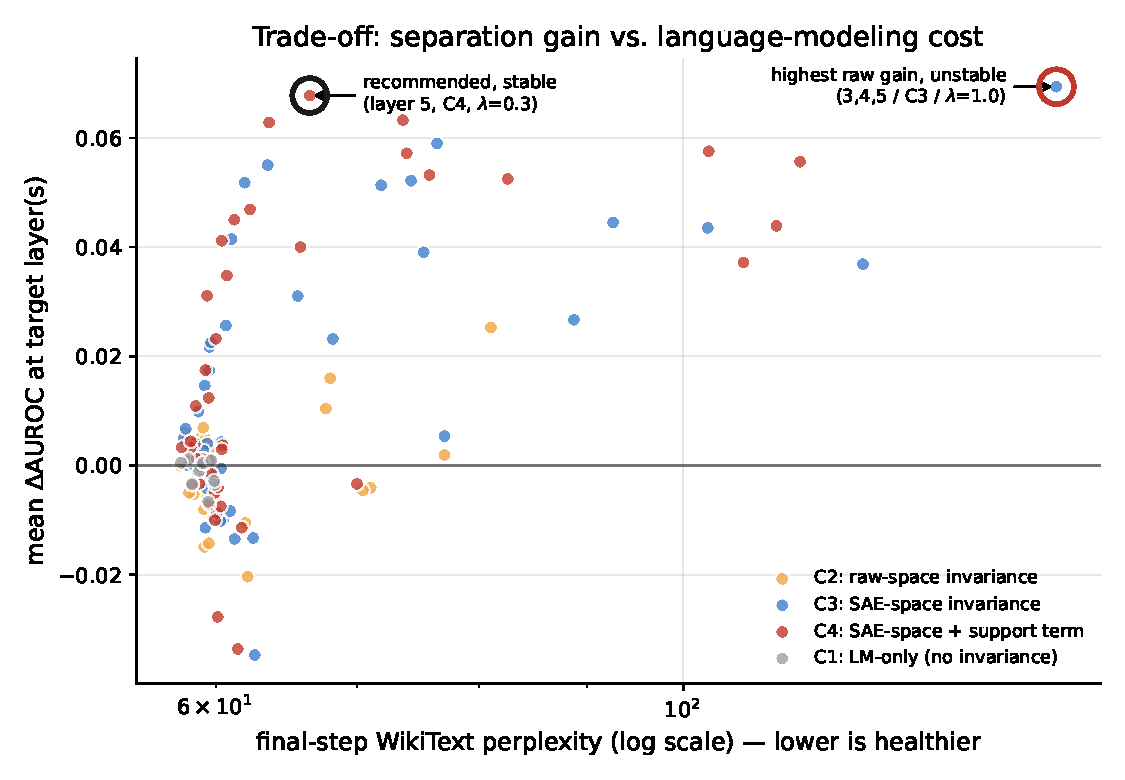
\includegraphics[width=0.8\textwidth]{tradeoff_gain_vs_perplexity}
\caption{مصالحهٔ میان بهبود \lr{AUROC} و سرگشتگی نهایی \lr{WikiText}، برای هر یک از ۱۶۰ اجرا. محور افقی لگاریتمی است. دایرهٔ توخالی مشکی، پیکربندی توصیه‌شده را نشان می‌دهد؛ دایرهٔ توخالی قرمز، پیکربندی با بیشترین بهبود خام را.}
\label{fig:tradeoff}
\end{figure}

این نمودار، همان الگویی را که در سه بخش پیشین به‌صورت میانگین دیده شد، در سطح تک‌تک اجراها آشکار می‌کند: ابر نقاط خاکستری و نارنجی
(\lr{C1}
و
\lr{C2}) تقریباً همگی در نوار باریکی از سرگشتگی پایین و بهبود نزدیک به صفر متمرکزند. ابر نقاط آبی و قرمز
(\lr{C3}
و
\lr{C4}) اما، یک الگوی روشن نشان می‌دهند: با دورشدن به سمت راست نمودار (سرگشتگی بالاتر)، بهبود نیز افزایش می‌یابد، اما این افزایش
\emph{نزولی}
است--یعنی شکل ابر نقاط، بیشتر یک سطح صعودی رو‌به‌کاهش است تا یک خط راست. پیکربندی توصیه‌شده (دایرهٔ مشکی) دقیقاً در ناحیه‌ای از این ابر قرار دارد که به لبهٔ سمت چپ آن (سرگشتگی پایین) نزدیک است اما هنوز بهبودی نزدیک به بیشینهٔ کل نمودار به دست می‌دهد؛ پیکربندی با بیشترین بهبود خام (دایرهٔ قرمز) در انتهای دور راست همین ابر قرار دارد، جایی که برای رسیدن به کمترین مقدار اضافی بهبود، باید بهای سرگشتگی‌ای پرداخت که چند برابر بزرگ‌تر است. به‌عبارت دیگر، شکل~\ref{fig:tradeoff} به‌روشنی نشان می‌دهد که پیمودن کامل این منحنی تا انتهای آن، ارزش اقتصادی نزولی دارد: بخش عمدهٔ بهبود، با بخش کوچکی از هزینهٔ کل سرگشتگی به دست می‌آید.

\subsection{اعتبار بازسازی خودرمزگذار}
شکل~\ref{fig:fidelity} میانگین واریانس تبیین‌شدهٔ بازسازی را در گام پایانی آموزش، به‌تفکیک شرط و $\lambda$ نشان می‌دهد.

\begin{figure}[htb]
\centering
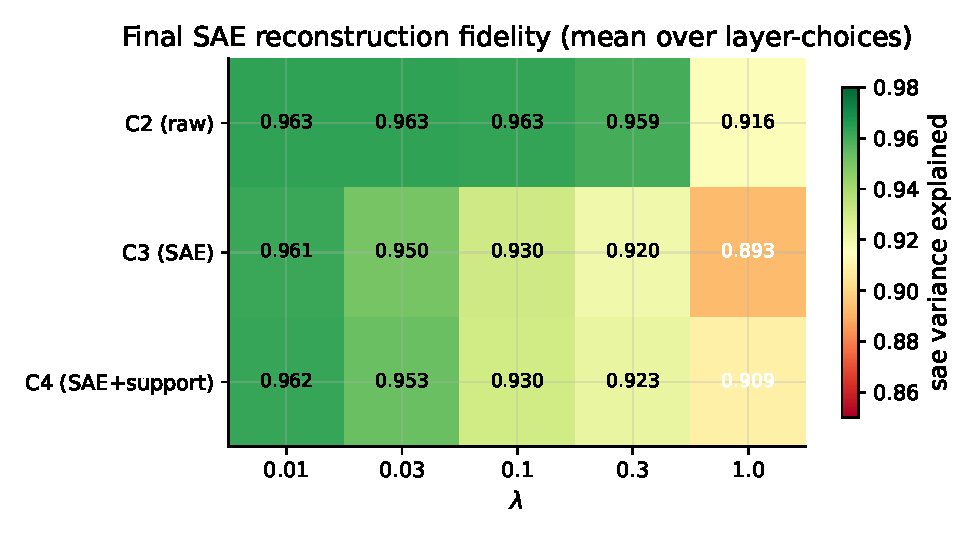
\includegraphics[width=0.7\textwidth]{fidelity_heatmap}
\caption{میانگین واریانس تبیین‌شدهٔ بازسازی خودرمزگذار در گام پایانی آموزش، به‌تفکیک شرط و $\lambda$ (میانگین روی هر ده حالت انتخاب لایه).}
\label{fig:fidelity}
\end{figure}

الگوی این شکل، الگوی جدول سرگشتگی را بازتاب می‌دهد: تا
$\lambda=0.1$، واریانس تبیین‌شده در تمام شرایط بالای
$95\%$
باقی می‌ماند؛ از
$\lambda=0.3$
به بعد، شرایط
\lr{C3}
و
\lr{C4}
افت محسوسی نشان می‌دهند (به ترتیب
$92.0\%$
و
$92.3\%$
در
$\lambda=0.3$)، و در
$\lambda=1.0$
شرط
\lr{C3}
از آستانهٔ هشدار عبور می‌کند
($89.3\%$). در سطح کل
۱۶۰
اجرا،
$18.8\%$
از آن‌ها (عمدتاً شرایط
\lr{C3}/\lr{C4}
با
$\lambda \geq 0.3$) با واریانس تبیین‌شدهٔ کمتر از آستانهٔ هشدار به پایان رسیده‌اند.

\subsection{نمونه‌ای از مصالحه: دو اجرای متضاد}
برای مشاهدهٔ ملموس این مصالحه در طول زمان، شکل~\ref{fig:dynamics} دو سنجه را در طول آموزش، برای دو اجرا مقایسه می‌کند: پیکربندی توصیه‌شدهٔ این پایان‌نامه (لایهٔ هدف منفرد پنجم، شرط
\lr{C4}، $\lambda=0.3$؛ معرفی کامل در بخش~\ref{sec:res-best})، و یک پیکربندی تهاجمی‌تر با بهبود خام اندکی بالاتر (لایه‌های هدف سوم تا پنجم به‌طور هم‌زمان، شرط
\lr{C3}، $\lambda=1.0$).

\begin{figure}[htb]
\centering
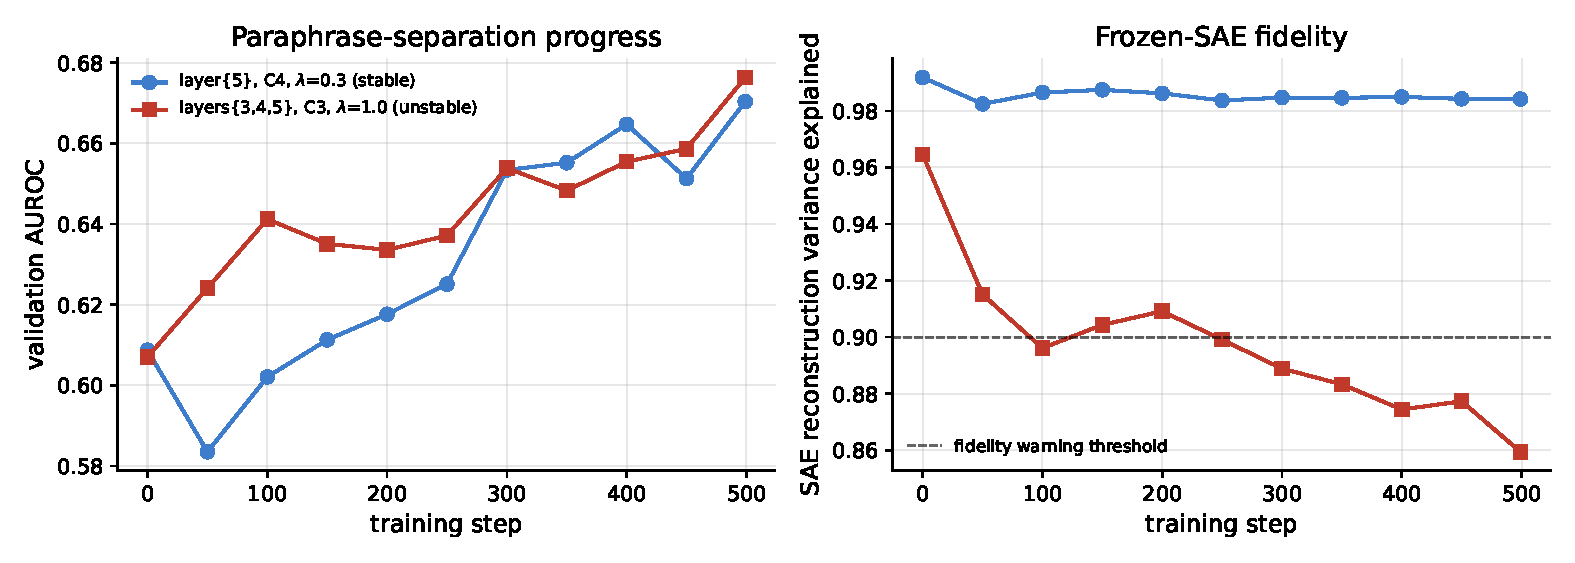
\includegraphics[width=0.95\textwidth]{training_dynamics}
\caption{پویایی آموزش برای پیکربندی توصیه‌شده (آبی) در برابر یک پیکربندی تهاجمی‌تر جایگزین با $\lambda=1.0$ و سه لایهٔ هدف هم‌زمان (قرمز). چپ: \lr{AUROC} اعتبارسنجی \lr{PAWS}. راست: واریانس تبیین‌شدهٔ بازسازی خودرمزگذار.}
\label{fig:dynamics}
\end{figure}

نمودار سمت چپ نشان می‌دهد که این دو پیکربندی به
\lr{AUROC} نهایی تقریباً یکسانی می‌رسند. نمودار سمت راست پیامد این تفاوت را برای اعتبار خودرمزگذار نشان می‌دهد: پیکربندی تهاجمی‌تر، در طول آموزش، پیوسته واریانس تبیین‌شدهٔ پایین‌تری دارد.

نتیجه‌گیری این مقایسه ساده است: دو پیکربندی به جداسازی تقریباً یکسانی می‌رسند، اما یکی از آن‌ها این کار را با هزینهٔ به‌مراتب کمتری--هم برای سلامت زبانی مدل و هم برای اعتبار ابزار سنجش--انجام می‌دهد. همین مشاهده، مبنای انتخاب پیکربندی توصیه‌شدهٔ بخش بعدی است.

\section{پیکربندی توصیه‌شده}
\label{sec:res-best}
با درنظرگرفتن هر سه سنجه--بهبود
\lr{AUROC}، سرگشتگی زبانی، و اعتبار بازسازی--پیکربندی توصیه‌شده،
\lr{C4}
با هدف‌گیری لایهٔ پنجم (تنها) و
$\lambda=0.3$
است. این پیکربندی به بهبود
$0.068$
در
\lr{AUROC} فضای
\lr{SAE}
می‌رسد--عملاً برابر با بالاترین بهبود خام کل شبکهٔ آزمایشی ($0.069$، متعلق به یک پیکربندی سه‌لایهٔ هم‌زمان با
$\lambda=1.0$)--درحالی‌که سرگشتگی نهایی‌اش
($66.5$)
تنها حدود
$13\%$
بالاتر از شرط کنترلی
($59.1$)
است و واریانس تبیین‌شدهٔ بازسازی‌اش
($98.4\%$)
به‌مراتب بالاتر از آستانهٔ هشدار باقی می‌ماند؛ در مقابل، پیکربندی سه‌لایهٔ
$\lambda=1.0$
سرگشتگی‌ای معادل
$150.3$
(بیش از دو ونیم برابر کنترل) و واریانس تبیین‌شده‌ای معادل
$86.0\%$
(زیر آستانهٔ هشدار) دارد. به‌عبارت دیگر، رفتن از
$\lambda=0.3$
به
$\lambda=1.0$
(به‌همراه افزودن دو لایهٔ هدف دیگر) تنها
$0.001$
واحد بهبود اضافی در
\lr{AUROC}
به همراه دارد، اما به بهای بیش از دو برابرشدن سرگشتگی و سقوط اعتبار خودرمزگذار به زیر آستانهٔ هشدار تمام می‌شود؛ مصالحه‌ای که ارزش آن سود اندک را ندارد.

% شکل~\ref{fig:profile} نمایهٔ کامل عمق این پیکربندی توصیه‌شده را در برابر خط پایه نشان می‌دهد.

% \begin{figure}[htb]
% \centering
% 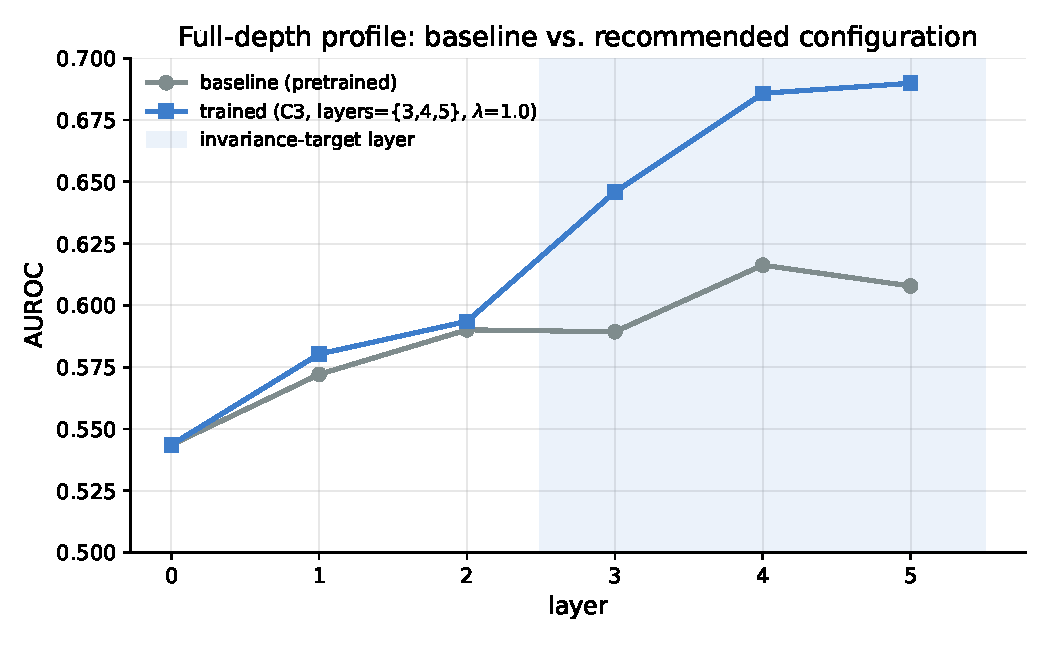
\includegraphics[width=0.85\textwidth]{profile_best_vs_baseline}
% \caption{نمایهٔ کامل \lr{AUROC} (فضای \lr{SAE}) در تمام لایه‌ها، برای خط پایه در برابر پیکربندی توصیه‌شده (\lr{C4}، لایهٔ هدف $\{5\}$، $\lambda=0.3$). ناحیهٔ سایه‌خورده، لایهٔ هدف را نشان می‌دهد.}
% \label{fig:profile}
% \end{figure}

% نکتهٔ مهم این نمایه، رفتار آن در لایه‌های \emph{غیرهدف} است: بهبود در لایه‌های ابتدایی مدل عملاً صفر است (نه مثبت و نه منفی محسوس)، اما در لایهٔ چهارم--که مستقیماً هدف قرار نگرفته، ولی بلافاصله \emph{پیش از} لایهٔ هدف قرار دارد--بهبود قابل‌توجه
% \lr{0.043}
% ثبت شده است. این «نشت» بهبود به‌سمت عقب، با معماری جریان باقیماندهٔ ترنسفورمر سازگار است: فعال‌سازی لایهٔ پنجم، تابعی مستقیم از فعال‌سازی لایهٔ چهارم است، و بنابراین، هر تغییری که وزن‌های لورا برای دورکردن بازنمایی لایهٔ پنجم اعمال می‌کنند، الزاماً بازنمایی لایهٔ چهارم (که ورودی لایهٔ پنجم را می‌سازد) را نیز تحت‌تأثیر قرار می‌دهد. این یافته پیشنهاد می‌کند که تعمیم اثر این روش، بیشتر «رو به عقب» (به لایه‌های نزدیک‌تر به ورودی که خروجی‌شان مستقیماً وارد لایهٔ هدف می‌شود) رخ می‌دهد تا «رو به جلو».

% \section{تحلیل تکمیلی: تمرکز سیگنال در فضای ویژگی‌ها}
% \label{sec:res-interp}
% به‌عنوان یک تحلیل اکتشافی و مکمل، سهم ویژگی‌های
% \lr{SAE}
% با بیشترین تغییر میان جفت‌جمله‌های هم‌معنی
% (\lr{top5pct\_latent\_share}؛ بخش~\ref{sec:metrics}) نیز برای پیکربندی توصیه‌شده اندازه‌گیری شد. شکل~\ref{fig:interp} این سنجه را برای خط پایه و برای پیکربندی توصیه‌شده مقایسه می‌کند.

% \begin{figure}[htb]
% \centering
% 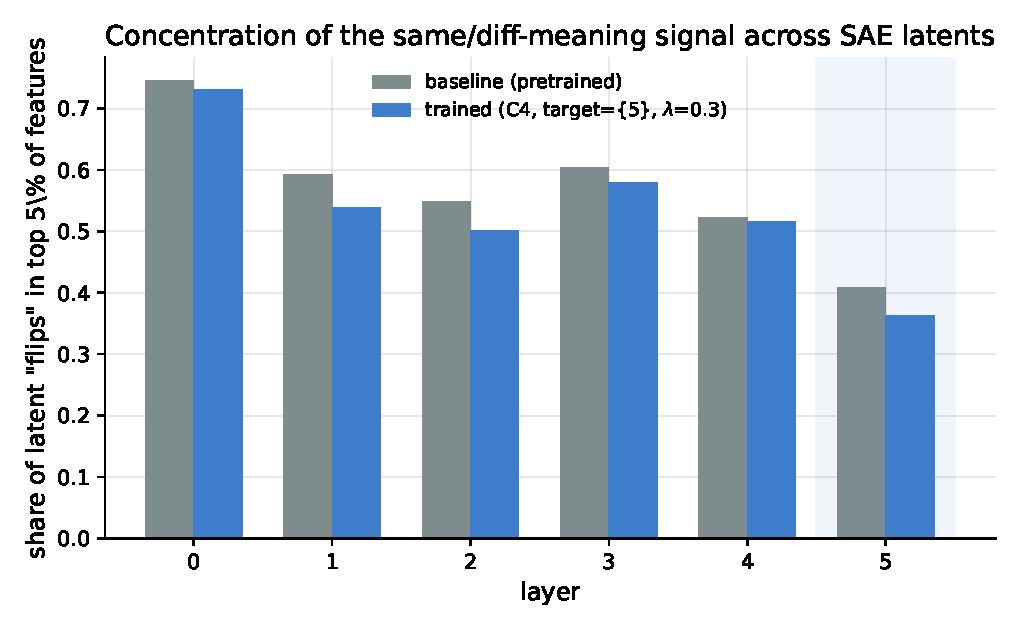
\includegraphics[width=0.8\textwidth]{latent_concentration}
% \caption{سهم ویژگی‌های \lr{SAE} با بیشترین تغییر میان جفت‌های هم‌معنی، در هر لایه؛ خط پایه در برابر پیکربندی توصیه‌شده.}
% \label{fig:interp}
% \end{figure}

% برخلاف پیکربندی‌های تهاجمی‌تر (که در بررسی‌های مقدماتی، الگویی ناهمگون از افزایش در برخی لایه‌ها و کاهش در برخی دیگر نشان می‌دادند)، پیکربندی توصیه‌شده--محافظه‌کارانه‌تر و محدود به یک لایهٔ هدف--اثری ملایم و تقریباً یکنواخت دارد: این سنجه در \emph{تمام} لایه‌ها، شامل لایه‌های غیرهدف، اندکی کاهش می‌یابد (برای نمونه، در لایهٔ هدف، از
% \lr{0.408}
% به
% \lr{0.363}). این پایان‌نامه از تعمیم این مشاهده به یک ادعای کلی دربارهٔ «تفسیرپذیرترشدن» یا «تفسیرناپذیرترشدن» مدل پرهیز می‌کند؛ آنچه می‌توان با اطمینان گفت این است که تابع هزینهٔ ناوردایی، هیچ قید صریحی برای متمرکزکردن سیگنال در تعداد کمی ویژگی ندارد (چنین قیدی در طراحی تابع هزینه وجود ندارد)، و بنابراین هرگونه تغییر در این سنجه، اثر جانبی غیرمستقیم بهینه‌سازی است، نه هدف مستقیم آن؛ بررسی عمیق‌تر این پدیده--مثلاً با شناسایی دستی اینکه کدام ویژگی‌های خاص، سهم خود را تغییر داده‌اند--در این پایان‌نامه انجام نشده و به‌عنوان جهت پژوهش آینده در فصل پنجم مطرح می‌شود.

\section{جمع‌بندی نتایج}
یافته‌های این فصل را می‌توان در پاسخ به سه پرسش پژوهشی فصل اول این‌گونه خلاصه کرد. نخست، اعمال تابع هزینهٔ ناوردایی در فضای خودرمزگذار پراکنده، به‌طور پایدار و در سرتاسر شبکهٔ آزمایشی، جداسازی بهتری میان جفت‌جمله‌های هم‌معنی و ناهم‌معنی نسبت به اعمال همان تابع هزینه در فضای خام تولید می‌کند؛ شرط کنترلی فاقد هرگونه هدف ناوردایی، هیچ بهبودی نشان نمی‌دهد. دوم، این جداسازی به‌شدت به لایهٔ هدف (لایه‌های میانی-به-بعد، نه لایه‌های ابتدایی) و به وزن
$\lambda$
وابسته است، و اعمال هم‌زمان چند لایه اثری فراجمع‌شونده دارد. سوم، و مهم‌تر از نظر عملی: بالاترین بهبودهای خام--که همگی در
$\lambda$
بزرگ به دست می‌آیند--با هزینهٔ محسوسی در ثبات آموزش و در اعتبار خودرمزگذار همراه‌اند، درحالی‌که یک پیکربندی محافظه‌کارانه‌تر
($\lambda=0.3$، تک‌لایه) تقریباً به همان بهبود می‌رسد بدون تحمیل این هزینه. فصل پنجم این یافته‌ها را در پرتو اهداف پژوهش جمع‌بندی و محدودیت‌ها و جهت‌های پژوهش آینده را بیان می‌کند.
